\documentclass[12pt]{article}
\usepackage{pgf,tikz}
\usepackage{color}
\usepackage{amssymb}
\usepackage{amsmath}

\begin{document}

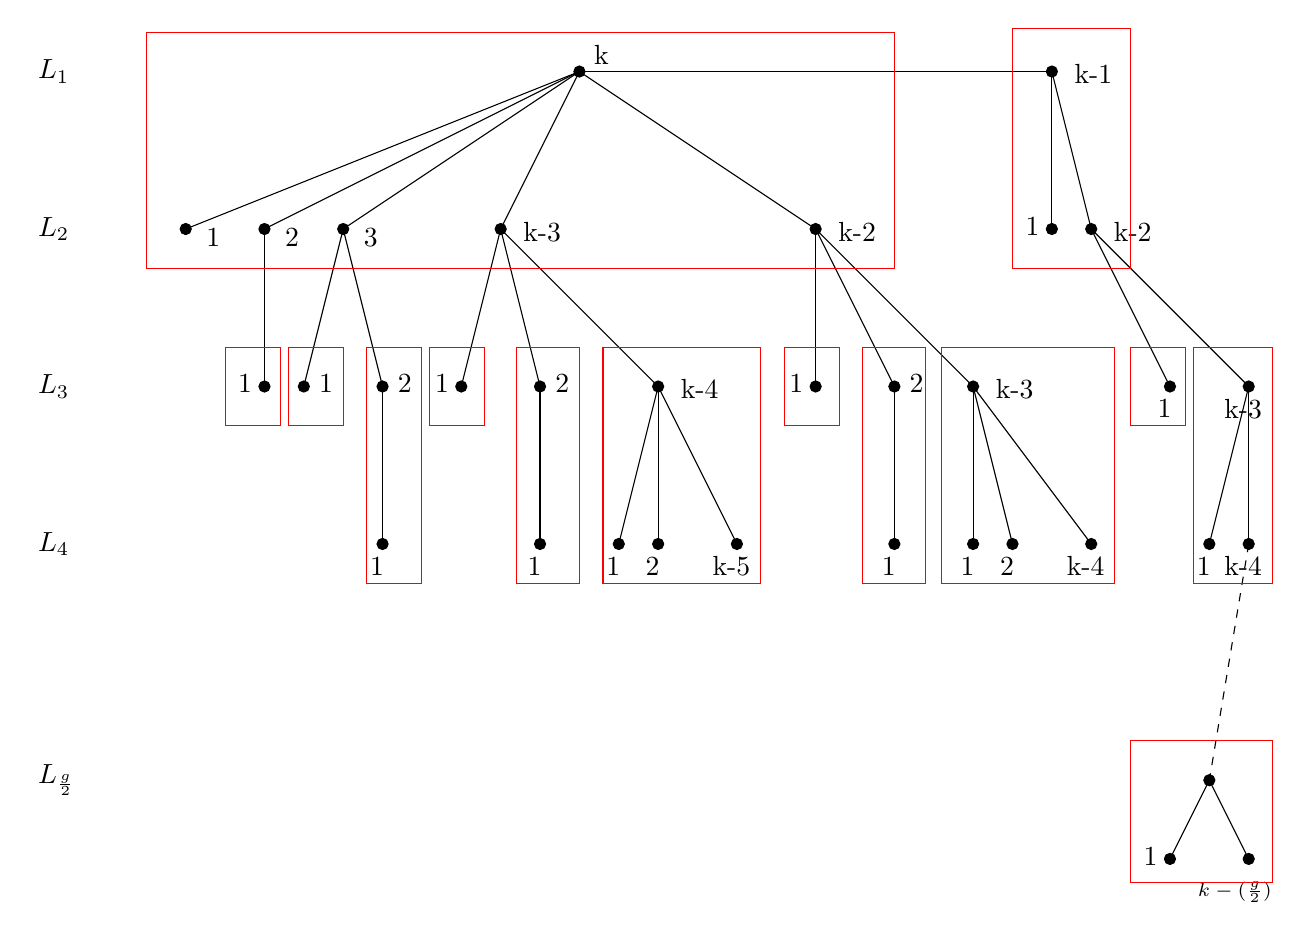
\begin{tikzpicture}
\filldraw (8,3) circle (2pt) node[xshift=8pt, yshift=6pt, scale=1pt]{k};
 %% level L2 point %%
\filldraw (3,1) circle (2pt) node[xshift=10pt, yshift=-3pt]{1};
\filldraw (4,1) circle (2pt) node[xshift=10pt, yshift=-3pt]{2};
\filldraw (5,1) circle (2pt) node[xshift=10pt, yshift=-3pt]{3};
\filldraw (7,1) circle (2pt) node[xshift=15pt, yshift=-1pt]{k-3};
\filldraw (11,1) circle (2pt) node[xshift=15pt, yshift=-1pt]{k-2};
\filldraw (14,3) circle (2pt) node[xshift=15pt, yshift=-1pt]{k-1};
%% line %%
\draw (8,3)--(3,1);
\draw (8,3)--(4,1);
\draw (8,3)--(5,1);
\draw (8,3)--(7,1);
\draw (8,3)--(11,1);
\draw (8,3)--(14,3);

%% level L3 point %%
\filldraw (4,-1) circle (2pt) node[xshift=-7pt, yshift=1pt]{1};
\filldraw (4.5,-1) circle (2pt) node[xshift=8pt, yshift=1pt]{1};
\filldraw (5.5,-1) circle (2pt) node[xshift=8pt, yshift=1pt]{2};
\filldraw (6.5,-1) circle (2pt) node[xshift=-7pt, yshift=1pt]{1};
\filldraw (7.5,-1) circle (2pt) node[xshift=8pt, yshift=1pt]{2};
\filldraw (9,-1) circle (2pt) node[xshift=15pt, yshift=-1pt]{k-4};
\filldraw (11,-1) circle (2pt) node[xshift=-7pt, yshift=1pt]{1};
\filldraw (12,-1) circle (2pt) node[xshift=8pt, yshift=1pt]{2};
\filldraw (13,-1) circle (2pt) node[xshift=15pt, yshift=-1pt]{k-3};
\filldraw (14,1) circle (2pt) node[xshift=-7pt, yshift=1pt]{1};
\filldraw (14.5,1) circle (2pt) node[xshift=15pt, yshift=-1pt]{k-2};
%% line %%
\draw (4,1)--(4,-1);
\draw (5,1)--(4.5,-1);
\draw (5,1)--(5.5,-1);
\draw (7,1)--(6.5,-1);
\draw (7,1)--(7.5,-1);
\draw (7,1)--(9,-1);
\draw (11,1)--(11,-1);
\draw (11,1)--(12,-1);
\draw (11,1)--(13,-1);
\draw (14,3)--(14,1);
\draw (14,3)--(14.5,1);

%% level L4 point %%
\filldraw (5.5,-3) circle (2pt) node[xshift=-2pt, yshift=-8pt]{1};
\filldraw (7.5,-3) circle (2pt) node[xshift=-2pt, yshift=-8pt]{1};
\filldraw (8.5,-3) circle (2pt) node[xshift=-2pt, yshift=-8pt]{1};
\filldraw (9,-3) circle (2pt) node[xshift=-2pt, yshift=-8pt]{2};
\filldraw (10,-3) circle (2pt) node[xshift=-2pt, yshift=-8pt]{k-5};
\filldraw (12,-3) circle (2pt) node[xshift=-2pt, yshift=-8pt]{1};
\filldraw (13,-3) circle (2pt) node[xshift=-2pt, yshift=-8pt]{1};
\filldraw (13.5,-3) circle (2pt) node[xshift=-2pt, yshift=-8pt]{2};
\filldraw (14.5,-3) circle (2pt) node[xshift=-2pt, yshift=-8pt]{k-4};
\filldraw (16,-3) circle (2pt) node[xshift=-2pt, yshift=-8pt]{1};
\filldraw (16.5,-3) circle (2pt) node[xshift=-2pt, yshift=-8pt]{k-4};
\filldraw (15.5,-1) circle (2pt) node[xshift=-2pt, yshift=-8pt]{1};
\filldraw (16.5,-1) circle (2pt) node[xshift=-2pt, yshift=-8pt]{k-3};
%% line %%
\draw (5.5,-1)--(5.5,-3);
\draw (7.5,-1)--(7.5,-3);
\draw (9,-1)--(8.5,-3);
\draw (9,-1)--(9,-3);
\draw (9,-1)--(10,-3);
\draw (12,-1)--(12,-3);
\draw (13,-1)--(13,-3);
\draw (13,-1)--(13.5,-3);
\draw (13,-1)--(14.5,-3);
\draw (14.5,1)--(15.5,-1);
\draw (14.5,1)--(16.5,-1);
\draw (16.5,-1)--(16,-3);
\draw (16.5,-1)--(16.5,-3);

%% level (g+1/2) point %%
\filldraw (16,-6) circle (2pt);
\filldraw (15.5,-7) circle (2pt) node[xshift=-7pt, yshift=1pt]{1};
\filldraw (16.5,-7) circle (2pt) node[xshift=-5pt, yshift=-12pt]{\scriptsize $k-(\frac{g}{2})$};
%% line %%
\draw (16,-6)--(15.5,-7);
\draw (16,-6)--(16.5,-7);
\draw[dashed] (16.5,-3)--(16,-6);
%% rectangle %%
\draw [{red}] (2.5,3.5) rectangle (12,.5);
\draw [{red}] (13.5,3.55) rectangle (15,0.5);
\draw [{red}] (3.5,-0.5) rectangle (4.2,-1.5);
\draw [{red}] (4.3,-0.5) rectangle (5,-1.5);
\draw [{red}] (5.3,-0.5) rectangle (6,-3.5);
\draw [{red}] (6.1,-0.5) rectangle (6.8,-1.5);
\draw [{red}] (7.2,-0.5) rectangle (8,-3.5);
\draw [{red}] (8.3,-0.5) rectangle (10.3,-3.5);
\draw [{red}] (10.6,-0.5) rectangle (11.3,-1.5);
\draw [{red}] (11.6,-0.5) rectangle (12.4,-3.5);
\draw [{red}] (12.6,-0.5) rectangle (14.8,-3.5);
\draw [{red}] (15,-0.5) rectangle (15.7,-1.5);
\draw [{red}] (15.8,-0.5) rectangle (16.8,-3.5);
\draw [{red}] (15,-5.5) rectangle (16.8,-7.3);

%% name level %%
\filldraw (1,3) circle (0pt) node[right]{$L_{1}$};
\filldraw (1,1) circle (0pt) node[right]{$L_{2}$};
\filldraw (1,-1) circle (0pt) node[right]{$L_{3}$};
\filldraw (1,-3) circle (0pt) node[right]{$L_{4}$};
\filldraw (1,-6) circle (0pt) node[right]{$L_{\frac{g}{2}}$};
\end{tikzpicture}

\end{document}